\documentclass[conference]{IEEEtran}

\usepackage[utf8]{inputenc} % allow utf-8 input
\usepackage[T1]{fontenc}    % use 8-bit T1 fonts
\usepackage{cite}
\usepackage[pdftex]{graphicx}
\usepackage{amsmath}
\usepackage{amsfonts}
\usepackage{amssymb}
\usepackage{mathtools}
\usepackage{array}
\usepackage{enumitem}
\usepackage{color}
\usepackage{url}
\usepackage[colorlinks=true,allcolors=black,urlcolor=blue]{hyperref}

%\usepackage{caption}
%\usepackage{subcaption}

%\captionsetup[figure]{textfont=footnotesize,labelfont=footnotesize}

\graphicspath{{images/}}
\DeclareGraphicsExtensions{.pdf,.jpeg,.png}
\interdisplaylinepenalty=2500

% Math commands for matrix and vector fonts
\providecommand{\v}{}
\renewcommand{\v}[1]{\underline{#1}}
\providecommand{\vhat}{}
\renewcommand{\vhat}[1]{\underline{\hat{#1}}}
\providecommand{\m}{}
\renewcommand{\m}[1]{{\bf #1}}
\providecommand{\j}{}
\renewcommand{\j}{\jmath}

% Custom math operators
\DeclareMathOperator*{\argmin}{arg\,min}
\DeclarePairedDelimiter\abs{\lvert}{\rvert}
\DeclarePairedDelimiter\norm{\lVert}{\rVert}
\DeclarePairedDelimiter\floor{\lfloor}{\rfloor}

\newcommand{\Phiorho}{\Phi\!\circ\!\rho}

\renewcommand*\ttdefault{lmtt}

% Theorems, lemmas, etc.
\newtheorem{theorem}{Theorem}
\newtheorem{lemma}[theorem]{Lemma}   % Shares numbering with theorem
\newtheorem{definition}{Definition}

% correct bad hyphenation here
%\hyphenation{op-tical net-works semi-conduc-tor}

\title{Minimax lower bounds for source localization}

\author{
	\IEEEauthorblockN{
		Praveen Venkatesh\IEEEauthorrefmark{1}
		and Pulkit Grover\IEEEauthorrefmark{2}
	}
	\IEEEauthorblockA{
		Electrical \& Computer Engineering,
		and the Center for the Neural Basis of Cognition,
		Carnegie Mellon University \\
		\IEEEauthorrefmark{1}\href{mailto:vpraveen@cmu.edu}{\texttt{vpraveen@cmu.edu}}
		\IEEEauthorrefmark{2}\href{mailto:pulkit@cmu.edu}{\texttt{pulkit@cmu.edu}}
	}
}

\begin{document}

\maketitle
\thispagestyle{plain}
\pagestyle{plain}

\begin{abstract}

The ``source localization'' problem is one that arises in several fields. For
instance, in neuroscience, one might wish to use electroencephalography (EEG)
measurements to locate the source of brain activity.
\textcolor{red}{<Briefly mention other applications>}.

The common underlying factor in each of these problems is the presence of a
point source, whose signal passes through a diffusive medium and is sensed by
an array of sensors. We then wish to recover the location of the source using
noisy sensed values. The diffusive medium is modeled as acting like a low-pass
filter. The noise is taken to be additive gaussian noise \textcolor{red}{which
may have a non-diagonal covariance matrix}.

\textcolor{red}{Rephrase this para.}
We give minimax lower bounds on the squared error in estimating the location of
the source, which applies to all estimators, when using unformly distributed
sensors and for certain classes of impulse response of the low-pass filter. Our
bounds are the first to give a scaling in terms of sensor density.

\end{abstract}

\section{Introduction}

%- The source localization problem is one that occurs in several fields
%  - Brain activity measurement, in the form of localizing brain activity
%    - Possible applications are epilepsy focus localization
%    - Neuroscientific experiments - locating the source of activity at certain
%      points in time, for understanding brain function
%  - Need to read Vetterli's papers on acoustic source localization-type things
%  - Need to read up linear inverse problems literature

%- Previous work
%  - In the brain activity localization side of things, lots of algorithms, but
%    not much understanding of bounds (Mosher, Grover).
%    - These have their own issues: CRLB does not apply to all estimators, info
%      theoretic bound does not give scaling with sensors
%  - Other work on minimax bounds and estimators for linear inverse problems
%    concentrate on function estimation (with smoothness constraints on the
%    function being estimated)
%    - e.g. Tsybakov, Efromovich, Ibragimov \& Has'minskii, and references
%      therein
%    - Obviously, bounds for function estimation will look radically different
%      from bounds for a location parameter
%    - Location-parameter based work appears to exist in Ibragimov-Has'minskii,
%      but they treat it as an exercise, without seriously considering
%      extensions, and looking at scaling with number of sensors

%- Cite Fisher's book on circular domain signals somewhere (statistical analysis
%  of circular data)

The source localization problem is one that appears in many fields where it is
of interest to find the position of a source (which emits some kind of signal)
using an array of sensors.

Our principal motivation comes from an application in brain activity
measurement, where one wishes to use modalities such as electroencephalography
(EEG) and magnetoencephalography (MEG) to record the activity inside the
brain~\cite{Baillet2001Electromagnetic}.  For example, current EEG systems use
anywhere between 10 and 250 sensors (electrodes), placed on the scalp, to sense
electric potentials produced by neuronal activity within the
brain~\cite{Nunez2006Electric}.

Recent developments~\cite{Grover2016Information} have suggested that source
localization can benefit greatly from an increase in sensor density. This
conclusion is based primarily on a Nyquist rate analysis, and on
information-theoretic bounds (which are possibly very loose) on the accuracy of
source localization algorithms. These bounds, first derived
in~\cite{Grover2016Fundamental}, do not capture scaling in number of sensors,
however, as the derivation effectively assumes the presence of an infinite
number of sensors to derive the bound.

Earlier work by Mosher et al.~\cite{Mosher1993Error}, which seeks to address
this issue by deriving Cramer-Rao lower bounds, is also not completely
satisfactory because these bounds do not apply to biased estimators. Commonly
used source localization algorithms (such as the Minimum Norm
Estimate~\cite{Hamalainen1994Interpreting}) on the other hand, are known to be
biased~\cite{Lin2006Assessing}.

This paper seeks to address the shortcomings of earlier methods by deriving
minimax lower bounds for the source localization problem, which apply to
\emph{all} estimators (biased \emph{and} unbiased), and which can give a
scaling in terms of the number of sensors used (for a fixed sensor placement
configuration). Computing the lower bound for the ``real brain model'' (where
the complete geometry of the brain surface is accounted for) is rendered very
difficult since analytical solutions for the EEG signal, given the brain
activity, do not exist. ``Spherical head
models''~\cite{Nunez2006Electric,Grover2016Information} \emph{do} have
analytical solutions, but are still not easily amenable to analytical lower
bounds because the spherical surface does not permit uniform
sampling~\cite{Heath1956Thirteen}, and because the solution is expressed in
terms of special functions. We therefore restrict our analysis to a source
localization problem on a one-dimensional domain (to be described in detail in
Section~\ref{sec:source-localization}).

The one-dimensional toy problem is an effective tool for understanding bounds
on source localization accuracy in other settings as well, such as
\textcolor{red}{<insert other applications>}. A vast literature on linear
inverse problems (refer~\cite{Bal2012Introduction} for an introduction to this
field) and deconvolution algorithms exists, and has addressed the reduced
one-dimensional problem in broad settings
(see~\cite{Cavalier2002Sharp,Efromovich1997Robust,Ibragimov1981Statistical} and
references therein). However, our setting and interpretation appears to be
unique, since most prior work focuses on recovering a whole function (given
certain smoothness constraints), rather than locating a point source. Work that
does address point sources, to our knowledge, does not address scaling in the
number of sensors, since their problem setting and application is very
different.

Hence, we believe that this paper is the first to give lower bounds on source
localization error (measured in an $ell_2$-distance sense) in estimating the
location of a one-dimensional point source, which is observed by sensors
through a diffusive medium (treated as a low-pass filter), and corrupted by
additive Gaussian noise. We describe the problem setting in detail in
Section~\ref{sec:source-localization}, describe the minimax technique used and
give our main result in Section~\ref{sec:minimax-lower-bounds}, describe a few
straightforward extensions in Section~\ref{sec:extensions}, and conclude with a
discussion on implications for sensor placement and future work in
Section~\ref{sec:discussion}.

%\textcolor{red}{Introduction needs to be re-written.}

%Electroencephalograhy (EEG) is a system used to record the electrical activity
%of the brain. It is a non-invasive system, which may use anywhere from around
%10 to 250 electrodes placed on the scalp, to sense electric potentials. These
%potentials are generated by neuronal activity within the
%brain~\cite{Buzsaki2012Origin}. These sources of neural activity -- neurons or
%groups of neurons -- are usually modeled as current
%dipoles~\cite{Nunez2006Electric}.

%Often, it is of clinical or scientific interest to reconstruct brain activity
%patterns from EEG sensor measurements. This process is what is broadly referred
%to when we speak of the term ``source localization''. In this paper, I restrict
%the discussion to that of localizing a \emph{single} dipole, and refer to this
%process as ``dipole source localization''. Several algorithms for source
%localization have been proposed over the years
%(see~\cite{Baillet2001Electromagnetic} for an excellent review). However, until
%recently, there has been only one work that has theoretically examined the
%fundamental limits of source localization accuracy.

%Mosher et.\ al.~\cite{Mosher1993Error} first propounded Cramer-Rao lower bounds
%for unbiased source localization algorithms. Their work also forms the basis
%for setting up the source localization problem and deriving more universally
%applicable bounds in this paper. The Cramer-Rao lower bound is not in itself a
%completely satisfactory answer to the question of fundamental limits for source
%localization accuracy. This is because Cramer-Rao bounds only apply to unbiased
%estimators (or to estimators of \emph{known} bias). In practice, however, many
%popular source localization algorithms have been shown to be biased, e.g.\
%the Minimum Norm Estimate (MNE)~\cite{Hamalainen1994Interpreting} is known to
%bias the solution towards the surface of the head~\cite{Lin2006Assessing}. It
%is also known that unbiased estimators can have worse mean-squared-error
%performance than biased estimators. So Cramer-Rao bounds are useful only to a
%degree, and there may be benefit in deriving bounds that hold for all
%estimators.

%To this end, Grover~\cite{Grover2016Fundamental} recently proposed a new lower
%bound for the error in localizing a single dipole. This bound used techniques
%from information theory, for bounding the source localization error by
%expressing it in terms of the mutual information across some channel, and then
%bounding the mutual information by the capacity of the channel. In deriving
%this bound, however, the scalp potential was never sampled; equivalently, it
%was assumed that an \emph{infinite} number of sensors was available to sample
%the EEG signal at every point on the scalp. Clearly, this is a poor assumption
%and could result in a very loose bound, because it allows for more information
%to be available at the receiver than otherwise possible. The lower bound also
%relies on certain relaxations that allow the dipole to distribute its power in
%non-physical ways in frequency domain. This once again makes the bound loose by
%assigning the channel a higher capacity than what it could otherwise have.

%To address the shortcomings of the Cramer-Rao and information theoretic lower
%bounds, I apply two minimax methods to the problem of computing a lower bound
%for localization error in the idealized EEG dipole source localization problem.
%I briefly review two minimax methods -- Le Cam's, and Fano's local
%method~\cite{Duchi2015Information} -- and describe my approach in deriving the
%minimax lower bound using each of these for spherical and one-dimensional head
%models.

\section{The source localization problem}
\label{sec:source-localization}

We start by giving a detailed description of the one-dimensional setting of the
source localization problem. Recall that, in this problem, we're trying to
determine the location of a point source by observing it through a diffusive
medium using a sensor array.

\subsection{Description of the domain}

We assume that the point source is located on a circle of circumference $T$ (a
circular domain enables us to use symmetry arguments to simplify the proof). We
can view this domain as a line, on which signals are periodic with period $T$.
The point source is therefore located somewhere within one period. We denote
the set of possible locations by $\Theta = [0, T)$. Due to the periodic nature
of the domain, a source located at position $\theta \in \Theta$ implies the
presence of sources at $t = \theta + kT$,~$\forall \, k \in \mathbb Z$.

\subsection{Sensor configuration}

Sensors are assumed to be uniformly distributed over the domain, i.e., if there
are $m$ sensors, they are placed at locations $t = 0$, $T/m$, $2T/m$,~\dots,
$(m{-}1)T/m$ (the offset of the first sensor is arbitrary, so without loss of
generality we take it to be 0). The periodicity of the space ensures that we
automatically also have sensors at $T$, $T{+}T/m$,~\dots\@ The lower bounds we
provide, therefore, are for \emph{this specific sensor configuration}. For a
discussion on why this configuration might be an appropriate choice in the
minimax setting, and on non-uniform sensor placement, see
section~\ref{sec:discussion}.

\subsection{Signal model}
\label{sec:signal-model}

All signals on the aforementioned circular domain are of the form
$f:\Theta\mapsto\mathbb{R}$.  The point source located at $\theta$ is
represented by the impulse signal, $f(t;\theta) = \delta(t - \theta)$, where
$\delta(\cdot)$ is the Dirac delta function.  The sensors observe this signal
through the diffusive medium, which, intuitively speaking, blurs the impulse.
More concretely, we assume that the medium is linear and shift-invariant, so
that it can be represented by a spatial impulse response (blurring would then
correspond to low-pass filtering). Let this impulse response be given by
$g(t)$. Then, the noiseless, continuous-space signal (post-filtering and
pre-sampling) is given by the convolution, $x(t; \theta) = (g*f)(t) = g(t -
\theta)$. Here, we further make the simplifying assumption that $g(t)$ has a
sufficiently restricted support, so that aliasing effects are avoided, and
$x(t; \theta)$ is always well-defined. To be precise, $g(t) = 0$ when $\abs{t}
> w/2$, where the ``width'' $w$ of the impulse response satisfies $w < T / 2$
(the reason for the factor of $1/2$ will become clear in a later section).

The sensors sample this continuous-space shifted impulse response, with some
additive noise. We denote the noiseless sampled version of $x(t; \theta)$ by
the $m$-length vector $\v x(\theta)$:
\begin{equation} \label{eq:sampled-signal}
	\v x(\theta) = \bigg[x(0; \theta), \ldots, x\Big(\frac{kT}{m}; \theta\Big), \ldots, x\Big(\frac{(m-1)T}{m}; \theta\Big)\bigg]^T
\end{equation}
where $m$ is the number of sensors and $k \in \{0, 1, \ldots, m-1\}$. The
additive noise is given by $\v \epsilon$ (to be described shortly), and the
noisy samples are represented by $\v y$:
\begin{equation} \label{eq:sensor-obs}
	\v y = \v x(\theta) + \v \epsilon
\end{equation}
The complete signal model described in this section is summarized in
Fig.~\ref{fig:signal-model}.

\subsection{Channel model}
\label{sec:channel-model}

The noise $\v \epsilon$, introduced in equation~\eqref{eq:sensor-obs}, is
the only source of uncertainty in the problem. For our purposes, we assume that
$\v \epsilon$ is zero-mean and Gaussian, $\v \epsilon \sim \mathcal{N}(\v 0, \m
\Sigma)$. Two kinds of covariance matrices are of particular interest. The
first is dubbed the ``sensor noise'' setting, wherein $\m\Sigma = \sigma^2 \m
I$, i.e. the sensors are afflicted by i.i.d.\ noise. The second is called the
``source noise'' setting, wherein $\m\Sigma$ has off-diagonal terms.
\textcolor{red}{Insert description of source noise.}

With the addition of Gaussian noise, each possible source location $\theta$
gives rise to a different distribution at the sensors, denoted by
\begin{equation} \label{eq:p-theta}
	P(\theta) = \mathcal{N}(\v x(\theta), \m \Sigma).
\end{equation}
$\v y$ is therefore one sample from $P(\theta)$. The space of distributions
produced by all possible source locations is $\mathcal{P} = \{P(\theta) :
\theta \in \Theta \}$. We are interested in computing lower bounds for the loss
function $\Phi(\rho(\theta, \hat\theta)) = \abs{\theta - \hat\theta}^2$, where
$\hat\theta$ is some estimate of the location based on $n$ trials (i.e. $n$
realizations) of the noisy sensor observations $\v y$.

\begin{figure}[tp] %  figure placement: here, top, bottom, or page
	\centering
	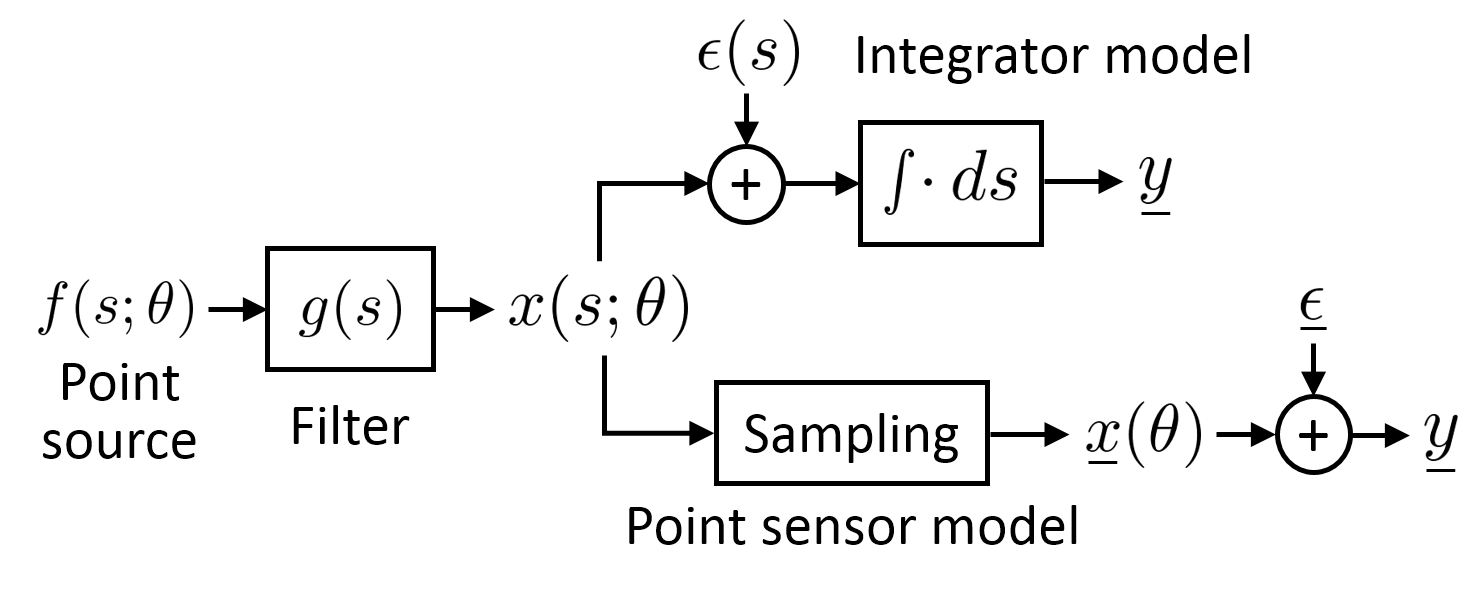
\includegraphics[width=3.5in]{block-diagram}
	\caption{A diagramatic representation of the signal model described in
	section~\ref{sec:signal-model}.}
	\label{fig:signal-model}
\end{figure}

\section{Minimax lower bounds for the one-dimensional model}
\label{sec:minimax-lower-bounds}

\subsection{Preliminaries}

We follow the excellent tutorial given in~\cite{Duchi2015Information} to
outline the preliminary steps in deriving bounds on the minimax risk.

Consider the following estimation problem: we have $n$ i.i.d.\ random samples
$Y^n$ from a distribution $P$, which is indexed by a parameter $\theta \in
\Theta$.  Denote the set of these distributions by $\mathcal{P} = \{P(\theta) :
\theta \in \Theta\}$. Suppose we now wish to estimate $\theta$ from $Y^n$.
Define a loss metric $\rho(\theta, \hat\theta)$ (e.g.\ $\rho(\theta,
\hat\theta) = \abs{\theta - \hat\theta}$). For this metric, we can define the
minimax risk over all possible estimators $\hat\theta(Y^n)$ and all possible
$\theta \in \Theta$:
\begin{equation} \label{eq:minimax-expr}
	\mathfrak{M}_n(\mathcal{P}, \Phiorho) = \inf_{\hat\theta} \sup_{\theta \in \Theta} \mathbb E[\Phiorho (\hat\theta(Y^n), \theta)]
\end{equation}
where $\Phi$ is any non-decreasing function (e.g.\ $\Phi(\rho) = \rho^2$) and
$Y^n$ is the random vector corresponding to a noisy realization of sensor
values.

We start by lower bounding the minimax risk of the estimation problem with the
risk incurred in a multiple hypothesis testing problem. For this, we first need
to define a $2\delta$-packing:%
\begin{definition}
	A set $\Theta_{\mathcal{V}} = \{ \theta_v : v \in \mathcal{V} \}$ for some
	finite index set $\mathcal{V} \subset \mathbb N$ is said to be a
	$2\delta$-packing in the $\rho$-metric if $\rho(\theta_i, \theta_j) \geq
	2\delta \, \forall \, \theta_i, \theta_j \in \Theta_{\mathcal{V}}$.
\end{definition}
\begin{theorem} \label{thm:est-to-testing}%
	If we can find a $2\delta$-packing $\Theta_{\mathcal{V}}$ of $\Theta$, then
	we can lower bound the minimax estimation risk by the average testing risk:
	\begin{equation}
		\mathfrak{M}_n(\mathcal{P}, \Phiorho) \geq \Phi(\delta) \inf_\psi \mathbb P (\psi(Y^n) \neq V)
	\end{equation}
	where $V$ is the unknown, true hypothesis, and $\psi$ is our estimate of
	the hypothesis.
\end{theorem}
For a proof of this theorem, we refer the reader to Proposition~13.3
in~\cite{Duchi2015Information}.  Intuitively, Theorem~\ref{thm:est-to-testing}
says that the error in estimating $\theta_i$ is likely to be more if it is
difficult to distinguish $\theta_i$ from $\theta_j$, i.e.\ if the probability
of error is high (where $\theta_j$ has been selected to be suitably close).

We now need to lower bound the probability of error in the hypothesis testing
problem. The simplest way to do this is to consider a binary hypothesis test
($\abs{\mathcal{V}} = 2$) and use what is known as Le Cam's method:
\begin{theorem} \label{thm:le-cam}
	For a binary hypothesis test, i.e., when $\mathcal{V} = \{0, 1\}$,
	\begin{equation}
		\inf_\psi \mathbb P(\psi(Y^n) \neq V) = 1 - \norm{P_0 - P_1}_{TV}
	\end{equation}
	where $P_i$ is short-hand for $P(\theta_i)$ and $\norm{P_0 - P_1}_{TV}$ is
	the total variation distance between the two distributions, defined as
	$\norm{\cdot}_{TV} = \frac{1}{2} \norm{\cdot}_1$.
\end{theorem}
For a proof, we refer the reader to Proposition~2.11
in~\cite{Duchi2015Information}.  Intuitively, Theorem~\ref{thm:le-cam} states
that the minimum probability of error that any estimator must make in a binary
hypothesis testing problem is related to the distance between the distributions
corresponding to the two hypotheses. The closer the two distributions, the
higher the chance of making an error in distinguishing between them.

Thus, the final lower bound can be written as:
\begin{equation} \label{eq:le-cam-bound}
	\mathfrak{M}_n(\mathcal P, \Phiorho) \geq \frac{\Phi(\delta)}{2} \big(1 - \norm{P_1^n - P_0^n}_{TV}\big)
\end{equation}
The superscripts ``$n$'' remind us that these are $n$-fold product
distributions, since we have $n$ i.i.d. trials used in the estimate.  The
difficulty in Le Cam's method lies in selecting the two hypotheses to trade-off
the effect due to a small value of $\delta$ and a large value of $\norm{P_1^n -
P_0^n}_{TV}$ appropriately, to derive the tightest possible bound.

\subsection{Lower bounds using Le Cam's method}

We now state the main result of this paper.
\begin{theorem}
	For a source localization problem as defined in
	section~\ref{sec:source-localization} with sensor noise and a spatial
	impulse response that is $\kappa$-Lipschitz continuous and has restricted
	support of width $w$, the asymptotic minimax risk in estimating the
	location of a point source is lower bounded by:
	\begin{equation}
		\mathfrak{M}_n(\mathcal{P}, \Phiorho) \geq \frac{1}{128} \frac{\sigma^2 T}{nm\kappa^2w}
	\end{equation}
\end{theorem}

\begin{IEEEproof}
Starting from equation~\eqref{eq:le-cam-bound} and working on the setting
described in Section~\ref{sec:source-localization}, we proceed to derive the
total variation distance for the distributions of interest. Using Pinsker's
inequality~\cite{Kullback1967Lower} and the convenient tensorization of the
KL-divergence~\cite{Duchi2015Information}, we see that:
\begin{equation} \label{eq:pinsker-tensorization}
	\norm{P_1^n - P_0^n}_{TV}^2 \leq \frac{1}{2} D_{KL}(P_0^n \Vert P_1^n) = \frac{n}{2} D_{KL}(P_0 \Vert P_1)
\end{equation}
For multivariate normal distributions with the same covariance, the
KL-divergence is given by
\begin{equation} \label{eq:kl-div-normal}
	D_{KL}(P_0 \Vert P_1) = (\v \mu_0 - \v \mu_1)^T \m \Sigma^{-1} (\v \mu_0 - \v \mu_1)
\end{equation}
where $\v \mu_0$ and $\v \mu_1$ are the means of $P_0$ and $P_1$
respectively~\cite{DuchiDerivation}.

\begin{figure}[t]
	\centering
	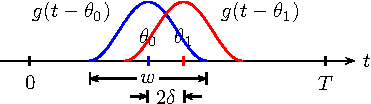
\includegraphics[width=2.8in]{overlap-middle-pics}
	\caption{Depiction of the continuous-space signals produced by two
		hypotheses, $\theta_0$ and $\theta_1$. Note that each signal is a
		shifted impulse response, and therefore has a support of size $w$.
		The set $\{\theta_0, \theta_1\}$ is a $2\delta$-packing of
		$\Theta$, so the signals are separated by a distance $2\delta$.}
	\label{fig:overlap-middle}
\end{figure}

\begin{figure}[t]
	\centering
	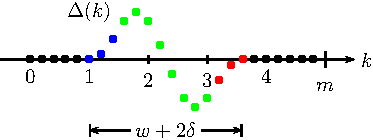
\includegraphics[width=2.8in]{delta-sampled-pics}
	\caption{Plot of the samples of the difference signal, $\Delta(k)$. The
		total size of the support of the difference signal is $w+2\delta$,
		hence at most $\floor*{\frac{(w + 2\delta)m}{T}}$ samples of
		$\Delta(k)$ are non-zero.}
	\label{fig:delta-sampled}
\end{figure}

For the case of sensor noise, $P_i = \mathcal{N}(\v x(\theta_i), \sigma^2 \m
I)$, as described in section~\ref{sec:channel-model}. Hence, combining
equations~\eqref{eq:le-cam-bound}, \eqref{eq:pinsker-tensorization} and
\eqref{eq:kl-div-normal}, we see that
\begin{equation} \label{eq:lb-after-pinsker}
	\mathfrak{M}_n(\mathcal{P}, \Phiorho) \geq \frac{\delta^2}{2} \Bigg[ 1 - \sqrt{ \frac{n}{2\sigma^2} \norm*{\v x(\theta_0) - \v x(\theta_1)}^2 } \Bigg]
\end{equation}
Let $\v \Delta \overset{\text{def.}}{=} \v x(\theta_0) - \v x(\theta_1)$ for
brevity. Also, let $\Delta(k)$ denote the $k$-th element of $\v\Delta$, and
$\mathbb I_A(k)$ denote the indicator function of $k$ belonging to the set $A$
(i.e., $\mathbb I_A(k) = 1$ if $k \in A$, and is $0$ otherwise). Then, we have
\begin{align}
	&\norm{\v\Delta}^2 = \sum_{k=0}^{m-1} \abs{\Delta(k)}^2 = \sum_{k=0}^{m-1} \abs{\Delta(k)}^2 \, \mathbb I_{\{\ell: \abs{\Delta(\ell)} > 0\}}(k) \\
	&= \sum_{k=0}^{m-1} \abs[\Big]{x\Big(\frac{kT}{m}; \theta_0\Big) - x\Big(\frac{kT}{m}; \theta_1\Big)}^2 \mathbb I_{\{\ell: \abs{\Delta(\ell)} > 0\}}(k) \\
	&= \sum_{k=0}^{m-1} \abs[\Big]{g\Big(\frac{kT}{m} - \theta_0\Big) - g\Big(\frac{kT}{m} - \theta_1\Big)}^2 \mathbb I_{\{\ell: \abs{\Delta(\ell)} > 0\}}(k)
\end{align}
where $x(t;\theta_i)$ is the continuous-space filtered signal described in
section~\ref{sec:signal-model}. For an impulse response $g$ which is Lipschitz
continuous with parameter $\kappa$, we can upper bound the term within the
summation:
\begin{equation}
	\abs[\Big]{g\Big(\frac{kT}{m} - \theta_0\Big) - g\Big(\frac{kT}{m} - \theta_1\Big)} \leq \kappa \abs{\theta_0 - \theta_1} = \kappa \cdot 2\delta
\end{equation}
since $\abs{\theta_0 - \theta_1} = 2\delta$ by virtue of the $2\delta$ packing.
Hence,
\begin{equation}
	\norm{\v\Delta}^2 \leq 4 \kappa^2 \delta^2 \sum_{k=0}^{m-1} \mathbb I_{\{\ell: \abs{\Delta(\ell)} > 0\}}(k) = 4 \kappa^2 \delta^2 \norm{\v\Delta}_0.
\end{equation}
$\norm{\v\Delta}_0$ is the number of non-zero elements in $\v\Delta$, which is
equal to the number of sensors in the total region covered by the signals
$x(t;\theta_0)$ and $x(t;\theta_1)$ (see Figs.~\ref{fig:overlap-middle} and
\ref{fig:delta-sampled}). Therefore, $\norm{\v\Delta}_0 = \floor[\big]{\frac{(w
+ 2\delta)m}{T} + 1}$, since at most a fraction $(w + 2\delta) / T$ of the $m$
sensors (plus 1, to account for edge-effects) can lie in the region covered by
the two impulse responses. The final upper bound on $\norm{\v\Delta}^2$ is
hence
\begin{equation} \label{eq:delta-bound}
	\norm{\v\Delta}^2 \leq 4 \kappa^2 \delta^2 \floor*{\frac{(w + 2\delta)m}{T} + 1} \leq 4 \kappa^2 \delta^2 \Big(\frac{(w + 2\delta) m}{T} + 1\Big).
\end{equation}
Since sensors are uniformly distributed, and since the domain is periodic, this
holds even if $\theta_0$ lies at the edge of the domain (close to $t=0$, for
example). In such a case, one part of the signal $x(t;\theta_0)$ will appear at
the left edge of the domain, and the repetition from the period $[T, 2T)$ will
appear at the right edge of the domain. Also note that the two signals
$x(t;\theta_0)$ and $x(t;\theta_1)$ overlap at most once, since $w < T/2$, as
stated in section~\ref{sec:signal-model}.

The upper bound in~\eqref{eq:delta-bound} translates into a lower
bound for~\eqref{eq:lb-after-pinsker}:
\begin{align}
	\mathfrak{M}_n(\mathcal{P}, \Phiorho) &\geq \frac{\delta^2}{2} \Bigg[ 1 - \sqrt{\frac{n}{2\sigma^2 T} 4 \kappa^2 \delta^2 (w + 2\delta) m} \Bigg] \\
	&= \frac{\delta^2}{2} \Bigg[ 1 - \sqrt{\frac{2nm \kappa^2 \delta^2 (w + 2\delta)}{\sigma^2 T}} \Bigg] \label{eq:lb-after-delta-bound}
\end{align}
Asymptotically, we choose smaller values of $\delta$ for larger number of
sensors. Hence, neglecting terms of order $\delta^3$, we tighten the bound by
choosing $\delta$ as a function of the remaining variables in order to have
$\sqrt{\frac{2nm\kappa^2\delta^2 w}{\sigma^2 T}} = \frac{1}{2}$. This is
achieved for $\delta = \sqrt{\frac{\sigma^2T}{8nm\kappa^2 w}}$, so that for
$\Phi(\delta) = \delta^2$, equation~\eqref{eq:lb-after-delta-bound} becomes
\begin{equation}
	\mathfrak{M}_n(\mathcal{P}, \Phiorho) \geq \frac{1}{128} \frac{\sigma^2 T}{nm\kappa^2 w}.
\end{equation}
This completes the proof.
\end{IEEEproof}

\section{Extensions}
\label{sec:extensions}

\subsection{From a circular (periodic) domain to a linear (aperiodic) domain}

So far, we've relied on the presence of a circular domain for to make the
arguments in the proof. However, the most important requirement was that
\emph{all} parts of the impulse response should get \emph{sensed} uniformly.
So, if $\theta$ were restricted to the region $[0, T)$ (now on a linear,
non-periodic domain), and if sensors were available to sense the signal from
$[-w/2, T{+}w/2)$ (for an impulse response with restricted support as described
in section~\ref{sec:signal-model}), then the proof for sensor noise would still
fall through, albeit with slightly different constants.

\subsection{From Lipschitz to $\alpha$-Holder continuous impulse responses}

We can trivially expand the domain of impulse responses to which the lower
bound applies to include $\alpha$-Holder continuous functions. These are
functions which satisfy
\begin{equation}
	\abs{g(u) - g(v)} \leq \kappa \norm{u - v}^\alpha \, \forall \, u, v \in \text{dom} \; g
\end{equation}
for some constant $\kappa$, and for $\alpha > 0$.

\subsection{From a one-dimensional domain to a $d$-dimensional domain}

Another simple extension takes our problem from a one-dimensional setting to a
$d$-dimensional setting. Here, we would have $\v\theta \in [0, T)^d$, and the
$\ell_2$ loss function, $\Phiorho(\v\theta, \vhat\theta) = \norm{\v\theta -
\vhat\theta}^2$. Then, using Assouad's lemma~\cite{Tsybakov2009Introduction} in
the manner described in~\cite{Duchi2015Information}, we can split the minimax
risk along each of the $d$ dimensions, and bound each separately using Le Cam's
method.

\section{Discussion}
\label{sec:discussion}

\textcolor{red}{Needs rewrite.}

The reason that the local Fano method gives a poorer bound than Le Cam's method
is that we're using the local Fano method on a bounded domain, making $V$ as a
function of the packing size $\delta$.  It is evident even from examining
equations \eqref{eq:fano-lb} and \eqref{eq:mutual-info-kl-reln} that taking
just two hypotheses with a suitable separation will yield tighter bounds, since
the cardinality of the packing set $V$ will no longer be dependent on $\delta$.
This will allow us to make use of the expression in equation
\eqref{kl-vi-vj-final} to choose $\delta$, which will yield the rate we saw in
Le Cam's method. It is to be seen whether using the global Fano
method~\cite{Duchi2015Information} will improve the rate, or at least, the
constants that we attained with Le Cam's technique. A more rigorous treatment,
which finds an upper bound for the sum, rather than using integrals, so as to
give bounds for even moderate numbers of sensors is also delegated to future
work.

%\IEEEtriggeratref{8}

\bibliographystyle{IEEEtran}
\bibliography{IEEEabrv,references}

\end{document}
